\documentclass[a4paper,12pt]{report}

\usepackage{alltt, fancyvrb, url}
\usepackage{amssymb}
\usepackage{graphicx}
\usepackage{subfigure}
\usepackage{wrapfig}
\usepackage{algorithmic}
\usepackage[utf8]{inputenc}
\usepackage{fontenc}
\usepackage{amsmath,stmaryrd,mathtools,algorithm}
\usepackage{amssymb}
%\usepackage{amsfonts}
\usepackage{float}
\usepackage{hyperref}
\usepackage{listings}
\usepackage{url}

\usepackage[english]{cleveref}

\usepackage[english]{babel}

\newtheorem{definition}{Definition}[section]
\newcommand{\R}{\mathbb{R}}
\newcommand{\dd}{\cdot}

\title{Introduction to LLL\\``Cryptography''}
 
\author{Di Santi Giovanni}
\date{\today}

\begin{document}
 
\maketitle

\tableofcontents

\chapter{Introduction to Lattices}

\section{Vector Spaces}

\begin{definition}
    \textbf{Vector space}.
\end{definition}
A \texttt{vector space} $V$ is a subset of $\R^{m}$ which is closed under finite vector addition and scalar multiplication, with the property that

\begin{center}
   $a_1v_1 + a_2v_2 \in V$ for all $v_1,v_2 \in V$ and all $a_1,a_2 \in \R$
\end{center}

\begin{definition}
    \textbf{Linear Combinations}
\end{definition}

Let $v_1,v_2,\ldots,v_k \in V$. A \texttt{linear combination} of $v_1,v_2,\ldots,v_k \in V$ is any vector of the form

\begin{center}
    $\alpha_1v_1 + \alpha_2v_2 + \cdots + \alpha_kv_k$ with $\alpha_1, \ldots, \alpha_k \in \R$
\end{center}

\begin{definition}
    \textbf{Lineaer Independece}
\end{definition}

A set of vectors $v_1,v_2,\ldots,v_k \in V$ is \texttt{linearly independent} if the the only way to get

\begin{center}
    $a_1v_1 + a_2v_2 + \cdots + a_kv_k = 0$
\end{center}

is to have $a_1 = a_2 = \cdots = a_k = 0$.

\begin{definition}
    \textbf{Bases}
\end{definition}

Taken a set of linearly independent vectors $x = (v_1,\ldots,v_n) \in V$ we say that $x$ is a \texttt{basis} of $V$ if $\forall w \in V$ we can write

\begin{center}
    $w = a_1v_1 + a_2v_2 + \cdots + a_nv_n$
\end{center}

\begin{definition}
    \textbf{Vector's length}
\end{definition}

The vector's length or \texttt{Euclidean norm} of $v = (x_1, x_2, \ldots, x_m)$ is

\begin{center}
    $\lVert v \rVert = \sqrt{x_1^2 + x_2^2 + \cdots + x_m^2}$
\end{center}

\begin{definition}
    \textbf{Dot Product}
\end{definition}

Let $v, w \in V \subset \R^m$ and $v = (x_1, x_2, \ldots, x_m), w = (y_1, y_2, \ldots, y_m)$, the \texttt{dot product} of $v$ and $m$ is

\begin{center}
    $v \dd m = x_1y_1 + x_2y_2 + \cdots + x_my_m$

    or

    $v \dd m = \lVert v \rVert \lVert w \rVert \cos{\theta}$
\end{center}

where $\theta$ is the angle between $v$ and $w$ if we place the starting points of the vectors at the origin $O$.

\begin{figure}[!b]
    \centering
    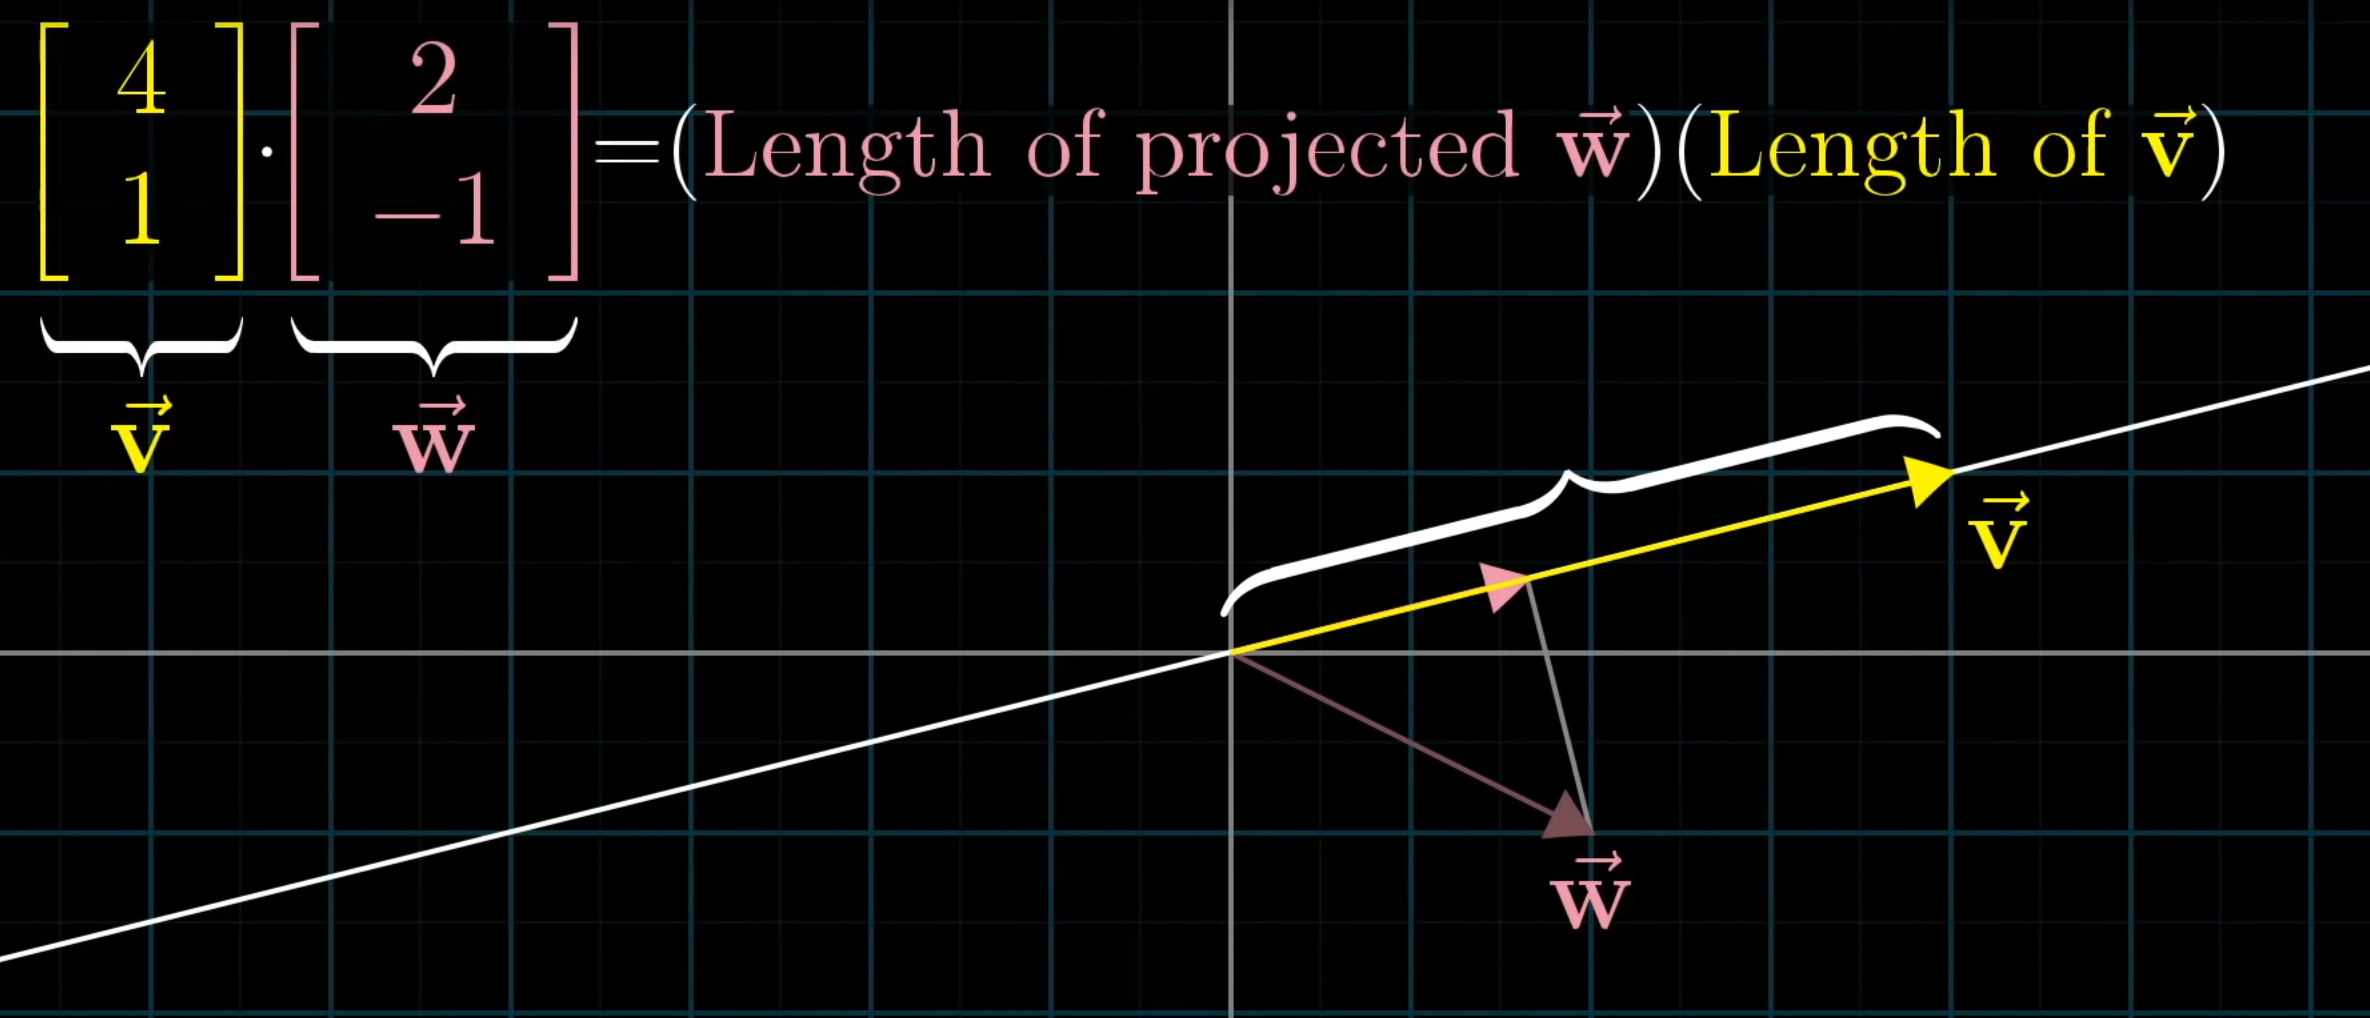
\includegraphics[scale=0.2]{./img/dot_product.png}
    \caption{Dot Product By 3Blue1Brown}
    \label{fig:dot_product}
\end{figure}

Geometrically speaking $v \cdot m$ is the length of $w$ projected to $v$ multiplied by the length of $v$ as shown in \ref{fig:dot_product}

\begin{definition}
    \textbf{Ortoghonal Basis} 
\end{definition}

An \texttt{ortoghonal basis} for a vector space $V$ is a basis $v_1, \ldots, v_m$ with the property that

\begin{center}
    $v_i \dd v_j = 0$ for all $i \neq j$
\end{center}

\section{Lattices}

\chapter{LLL}

\section{Purpose}

\section{Algorithm}

\chapter{Applications}

\section{Attack Knapsack}

\section{Attack RSA}

\chapter*{End of Paper}

$gg^2$

\bibliographystyle{plain}
\bibliography{paper}

\end{document}

